\startchapter{Experiment Results}
\label{chapter:results}

We devised six experiments to study the emergence of semantic representations 
in the brain during the symbol learning paradigm. We discuss these in order, 
beginning with the more fundamental experiments and ending with more detailed 
analyses built on those earlier experiments.

%\input chapters/4/sec_semanticrepresentation
  
\section{Semantic Representation Experiment} Here, we trained our model on a 
subset of the trials where we anticipated participant learning would have 
occurred, and evaluated this model with the 2 vs 2 test. Our model produced a 2 
vs 2 accuracy of \textbf{79.54\%} which is statistically above chance with $p < 
0.001$. This shows we can detect semantic representations in the brain using 
EEG data.

\section{Participant Learning Experiment} This experiment builds on the 
Semantic Representation Experiment, and aims to identify the trial at which we 
can detect meaning. Figure~\ref{fig:learning} plots the \tvt accuracy over 
trials.  When we average exposures (1, 2, 3) of each symbol, we achieve a  \tvt 
accuracy of \textbf{46.70\%}. Exposures (4, 5, 6) produce an accuracy of 
\textbf{72.35\%} with $p < 0.001$ (FDR corrected). Due to a reduction in data, 
the \tvt accuracy over trials (4, 5, 6) is slightly lower than the \tvt 
accuracy in the previous experiment, which used trials beyond the 6th exposure.  
This result confirms we can detect participant learning with our model.

\begin{figure}[t]
  \centering
  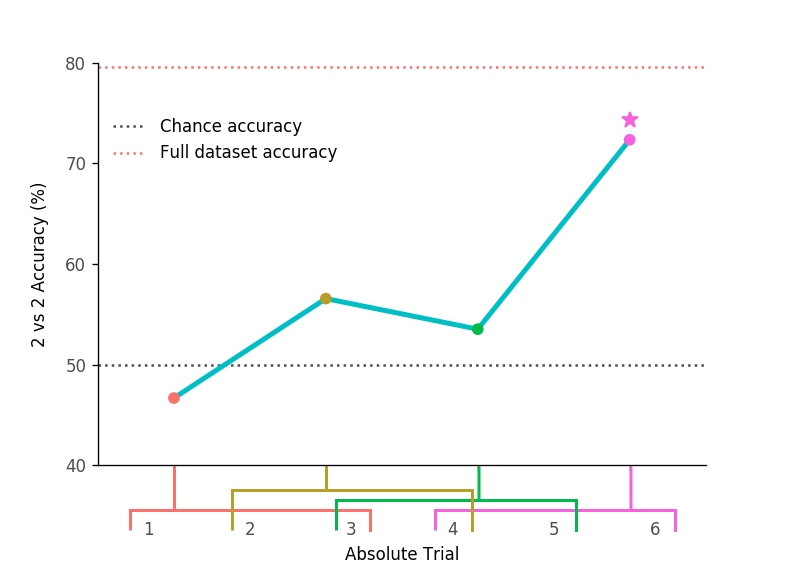
\includegraphics[width=0.75\linewidth]{figures/learning}
  \caption{A graph of 2 vs 2 accuracy over trials. This graphic shows how participant learning develops over time with a sliding window of three trial averages. 2 vs 2 accuracy increases notably in the last window, showing learning occurs in the later half of trials. A star indicates a statistically significant value with $p < 0.001$ (FDR corrected).}
  \label{fig:learning}
\end{figure}

\section{Reward Positivity Experiment} In order to compare our model with a 
more traditional ERP based analysis, here we analyze the reward positivity in 
the FCz electrode. We perform a comparison of the correct and incorrect 
responses as well as a comparison of the first six correct responses for a 
word.  Figure~\ref{fig:rewpos} shows the presence of reward positivity, 
confirmed by a dependent samples t-test of the difference waveform between the 
first correct response and the average of incorrect responses with $p < 0.001$.  
Figure~\ref{fig:rewpos_learning} shows the individual correct trials averaged 
over participants.  Here, we see a strong reward positivity for the first 
correct trial and a diminishing effect on subsequent correct trials (fitting a 
power law function with $R^2 = 0.96$). This confirms our hypothesis that the 
reward positivity decreases and the \tvt accuracy increases over trials.

\begin{figure}[t]
  \centerline{
    \includegraphics[width=\linewidth]{figures/rewpos}
  }
  \caption{The reward positivity for correct and incorrect responses at the FCz. In both graphics, the y-axis is positive downward. In {\bf A}, we see the signals of the averaged first correct trials for each word and all averaged incorrect trials. In {\bf B}, we see the difference between the averaged first correct trials and all averaged incorrect trials with 95\% confidence intervals. There is a clear presence of the reward positivity.}
  \label{fig:rewpos}
\end{figure}

\begin{figure}[t]
  \centerline{
    \includegraphics[width=\linewidth]{figures/rewpos_learning}
  }
  \caption{The reward positivity between the first six correct responses. The y-axis is positive downward for the left subfigure and positive upward for the right subfigure. In {\bf A}, we see the amplitude of the signal at the FCz electrode between the first six averaged correct responses. The amplitude of the correct waveform of the reward positivity is large on the first correct trial and diminishes with subsequent rewards. The change in this waveform indicates a diminishing reward positivity across learning. In {\bf B} we see the amplitude during the highest period of 228ms - 328ms after stimulus onset compared between the first six averaged correct responses. Again, here we see a clear reward positivity in the first correct trial and a diminishing effect on subsequent correct trials.}
  \label{fig:rewpos_learning}
\end{figure}

\section{Participant Performance Experiment} Here we test if the participants' 
\tvt accuracies are related to the participants' average task accuracies by 
examining the behavior data. The average task accuracy of individual 
participants ranges from 72\% - 90\% and the mean over all participants is 
81\%, and the standard deviation is 4\%. We split the participants into two 
groups based on their task accuracy, and evaluated the \tvt accuracy within 
these two groups. Because the variance of task accuracy is small across 
participants, we evaluated small groups of top and bottom performers. The 
average \tvt accuracy of the 7 participants with task accuracy below 80\% is 
{\bf 59.71\%}, and the \tvt accuracy of the 7 top participants (all above 85\% 
task accuracy) was {\bf 65.13\%}. While both of these \tvt accuracies are 
significantly lowered due to the reduction in training data compared to the 
previous two experiments, this suggests a relationship between task performance 
and our ability to detect the semantic meaning of the symbols via EEG.

\section{Time Windowing Experiment} The Time Windowing Experiment allows us to 
examine when the semantic representation in the brain is the strongest. The 
\tvt accuracy as a function of time \emph{within} an exposure is shown in 
Figure \ref{fig:timewindow}, allowing us to pinpoint the window where accuracy 
peaks. We find accuracy peaks in the 600ms-650ms window, at 74.57\% ($p < 
0.001$, FDR corrected). We also see an earlier spike which peaks in the 
150ms-200ms window, at 74.34\% ($p < 0.001$, FDR corrected).

\begin{figure}[t]
  \centering
  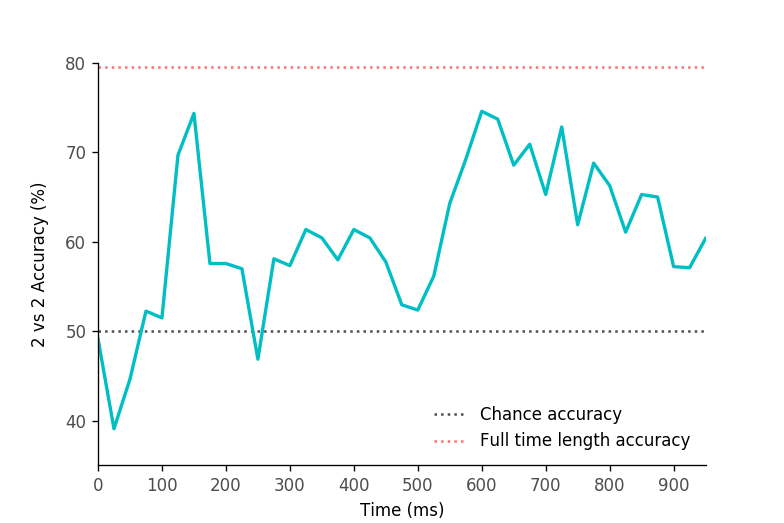
\includegraphics[width=0.75\linewidth]{figures/timewindow}
  \caption{A graph of 2 vs 2 accuracy over time. This graphic shows scores on the 2 vs 2 test evaluated with only the data present in 50ms incremental windows. For example, the point at 25ms defines the \tvt accuracy over the 25ms-75ms period. Statistically significant time windows are identified in red. The highest performing period is 600-650ms with 74.57\% accuracy ($p < 0.001$, FDR corrected). We also see an earlier spike which peaks at 150ms-200ms with 74.3\% accuracy ($p < 0.001$, FDR corrected).}
  \label{fig:timewindow}
\end{figure}

\section{Sensor Selection Experiment} Here we test which areas of the brain are 
contributing the most to the \tvt accuracy. We categorized sensors into $n_s$ 
groups for analysis, where each group consists of a primary sensor and its 
neighboring sensors. We used the accuracy of each sensor group to annotate the 
accuracy of the primary sensor, and then performed a topographic interpolation 
of the \tvt accuracy over the brain. The topographic interpolation of three 
time windows is visible in Figure~\ref{fig:topographic}. We see lower \tvt 
accuracies for the earlier time window (0-400ms) compared to the later time 
window (400ms-800ms), however we see the highest accuracies over the entire 
time window (0-1000ms).

\begin{figure}[t]
  \centering
  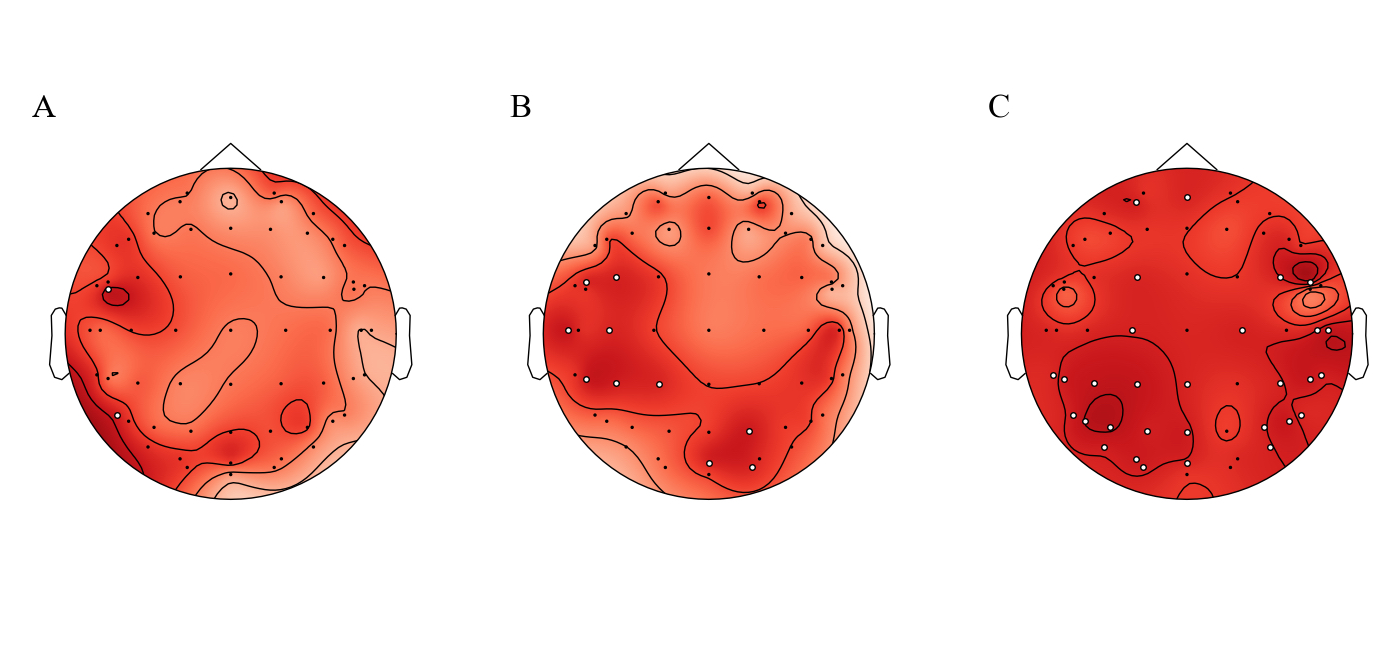
\includegraphics[width=0.9\linewidth]{figures/topographic}
  \caption{The results of the model on various brain regions. Each sensor represents a group containing it and its immediate neighbors, and we calculated \tvt accuracy using single groups.  A topographic plot of the \tvt accuracies is shown for three time periods: {\bf A}  0--400ms window; {\bf B} 400ms--800ms window; and {\bf C} 0--1000ms window. Statistically significant groups are shown in white ($p < 0.001$, FDR corrected).}
  \label{fig:topographic}
\end{figure}

\section{Conclusion}
contributing the most to the \tvt accuracy. We categorized sensors into $n_s$ 
groups for analysis, where each group consists of a primary sensor and its 
neighboring sensors. We used the accuracy of each sensor group to annotate the 
accuracy of the primary sensor, and then performed a topographic interpolation 
of the \tvt accuracy over the brain. The topographic interpolation of three 
time windows is visible in Figure~\ref{fig:topographic}. We see lower \tvt 
accuracies for the earlier time window (0-400ms) compared to the later time 
window (400ms-800ms), however we see the highest accuracies over the entire 
time window (0-1000ms).
